\documentclass[utf8]{webofc}
\usepackage[varg]{txfonts}
% review
\usepackage[textwidth=120]{todonotes}
%\usepackage{color}
\usepackage{subcaption}



\begin{document}
    \title{Calculation of gain coefficient in Dwyer relativistic discharge feedback model of thunderstorm runway breakdown}
    \author{\firstname{Mikhail} \lastname{Zelenyi}\inst{1,2,3}\fnsep\thanks{\email{mihail.zelenyy@phystech.edu}} \and
        \firstname{Egor} \lastname{Stadnichuk}\inst{1,2}\fnsep\thanks{\email{egrstadnichuk@yandex.ru}} \and \firstname{Alexander} \lastname{Nozik}\inst{1,2}\fnsep\thanks{\email{altavir@gmail.com}}  
    }
    
    \institute{Institute for Nuclear Research of RAS
        \and
        Moscow Institute of Physics and Technology (State University) 
        \and
        Space Research Institute of RAS
    }
    \abstract{%
        Terrestrial gamma flash (TGF) and thunderstorm ground enhancements(TGE) phenomena are crucial for understanding of atmosphere breakdown and lightning generation physics. The initial theory was developed by Gurevich and included only runway breakdown description. It was later updated by Babich and Dwayer, but even updated model uses a rather simplified field structure and does not fully match observed quantities. The reactor like TGE (RL-TGE) model presented in this work assumes more complicated stochastic field structure and takes into account not only one cell runway breakdown, but the whole global cell structure in the thundercloud. It allows to describe a wide variety of TGF-like events and potentially fills the gap in thundercloud parameters previously unaccounted by other theories.
    }
    %
    \maketitle
    
\section{Introduction}
% add intro   
    

\begin{figure}[b]
    % add description
	\centering
	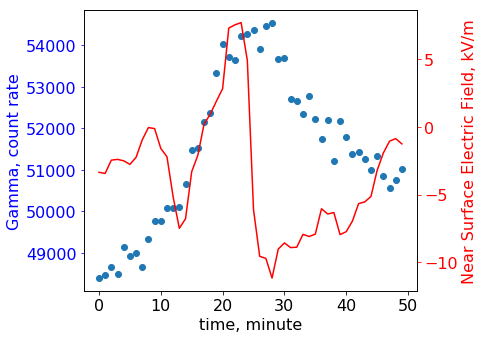
\includegraphics[width=0.5\textwidth]{figures/aragats.png}
	\caption{}
	\label{pic-aragats-a}   
\end{figure}        
\section{Reactor like TGE model}
Many previous works point to the fact that electric field inside the thundercloud is high enough to accelerate electrons and produce secondary electromagnetic showers ~\cite{gurevich1992runaway, gurevich1999lightning,dwyer2003fundamental,dwyer2011low}. The acceleration of electron is possible under two conditions:
\begin{itemize}
    \item The strength of the field is higher than so-called critical field. The value of the field equals energy loss of minimally ionizing electron per length unit.
    \item The initial electron energy is high enough to be close to minimally ionizing energy.
\end{itemize}
The major problem of all of these models is that that while field strength is higher than critical field, the multiplication coefficient for showers is rather small and can’t describe any observed effects.
The crucial part of this work is additional account for escaping high energy gamma-rays in the acceleration process. Escaping photons with energy higher than 1 MeV could produce (via photo-effect or compton-effect) new electrons with energy high enough to start separate acceleration process. These electrons are produced not in vicinity of first accelerator, but separated by free path of gamma ray which could amount up to few km. Thus these secondary accelerators could not be accounted by any local model. Additionally, the field map calculation shows that field directions in two points of a thundercloud separated by distances more than 500 m are mostly uncorrelated, meaning that direction of new accelerator is more or less random relative to the initial accelerator.
If the size of a thundercloud is much larger than mean free path of gamma-ray, one can observe a chain reaction, where photons are produced in elementary accelerator cells with given local multiplication coefficient depending on local field strength and then create additional elementary accelerator cells in separate places. Some of photons could be absorbed without creating additional cell. For example it could happen in case local field direction is opposed to photon and therefore produced electron momentum (<appendix with Egor’s calculations>). Accounting for such effects as well as loss of photons through borders of a thundercloud, one can get a global multiplicative coefficient. Obviously, in case global multiplication coefficient is larger than 1, one can observe an exponential rise in number of elementary accelerator cells and therefore total radiation level (gamma, infrared and neutron) and ionization. Also for coefficient slightly less than 1, one gets slow exponential decay of radiation background.
The described model is not unlike chain reaction process in nuclear reactor, so it could be called reactor-like terrestrial gamma enhancement model (RL-TGE).

\section{Proof of concept}
For fast checking the potential of our idea, we considered a next simplified model:  
\begin{itemize}
	\item There are only one tuning parameter  --- the local coefficient of gamma multiplication, describing usefulness of atmosphere for generating secondary particles;
	\item Production of Gamma in cell occurs by Poisson distribution, momentum direction of generated gamma is defined by the electric field direction;
	\item Electric field is chaotic: in point of cell ignition, direction of field is generated by uniform distribution, but magnitudes is constant for whole cloud;
	\item Energy of particle not taken into account, propagation of gamma simulated with exponential distribution with fixed mean free path;
	\item Cloud size is equals 1 kilometer and tracking of particle leaving volume stopped. 
\end{itemize}
This model is implemented as program on Kotlin\footnote{\url{https://kotlinlang.org/}} programming language.
    
\section{Results}
% add intro
The first figure shows the case of an explosive growth in the number of secondary photons that are well suited to the phenomenon of TGF.
The second figure demonstrates the case when there was a dissipation of an avalanche that had just begun to develop.
The third figure demonstrates the case of a slower and less intensive growth. Such processes with some minor adjustments and assumptions about field dynamics could describe TGE phenomenon.
    
\begin{figure}[ht!]
	\begin{subfigure}[b]{0.5\textwidth}
		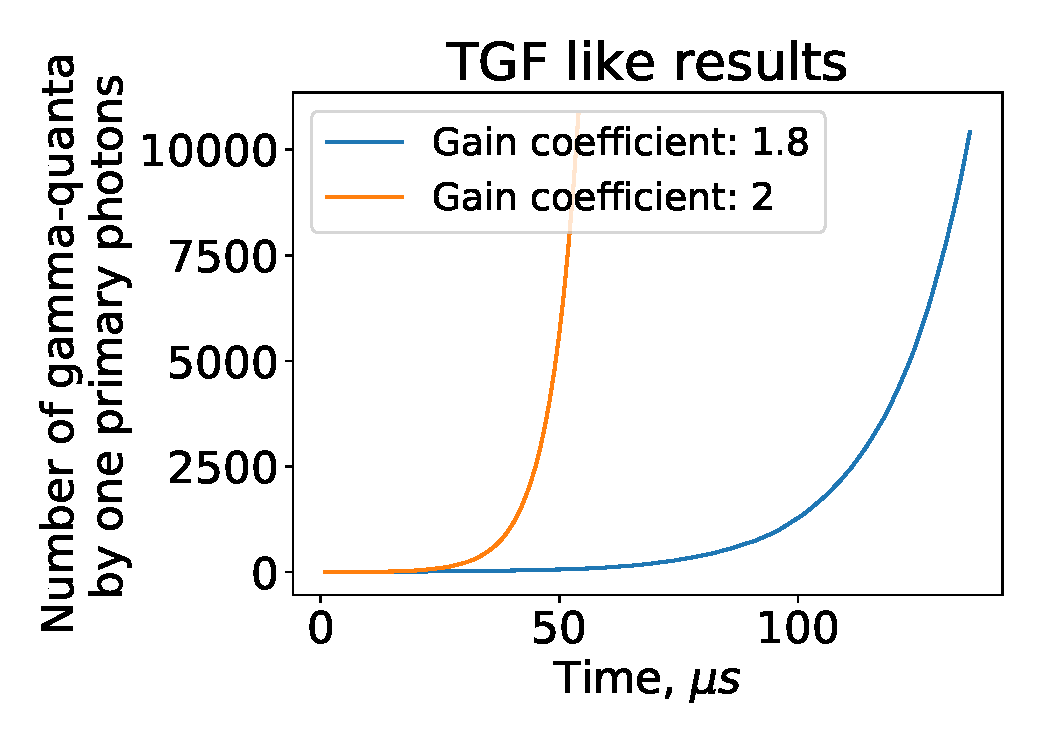
\includegraphics[width=0.95\linewidth]{figures/proofTGF.pdf}
		\caption{}
		\label{pic-tgf-a}
	\end{subfigure}
	~
	\begin{subfigure}[b]{0.5\textwidth}
		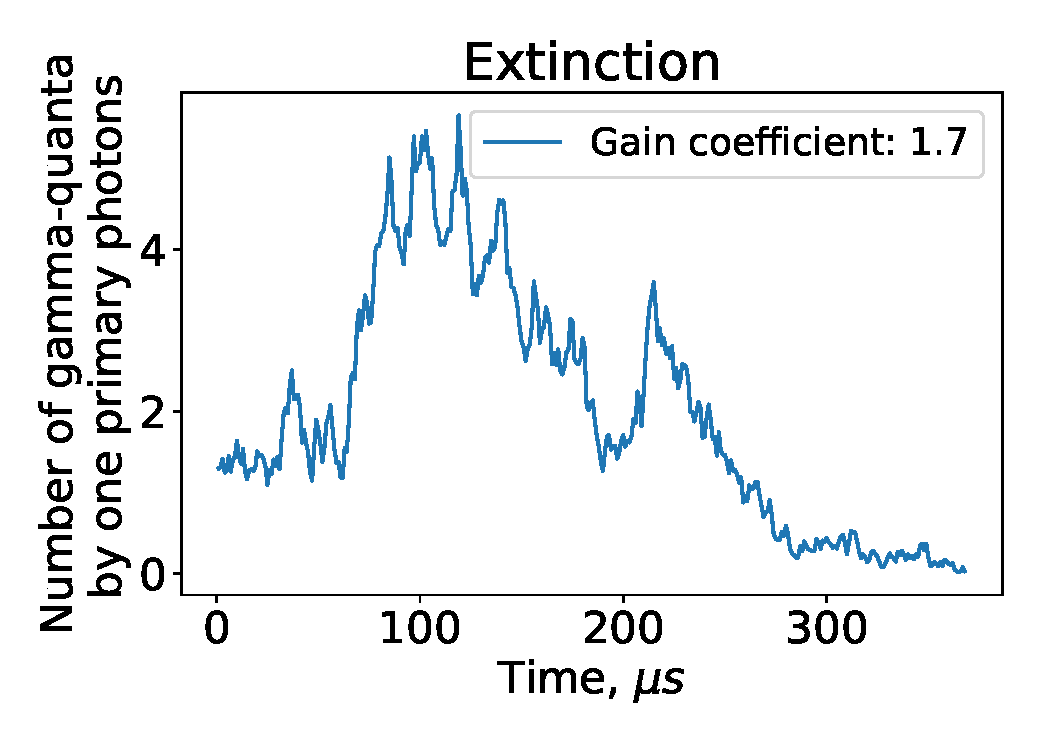
\includegraphics[width=0.95\textwidth]{figures/Extinction.pdf}
		\caption{}
		\label{pic-ext-b}
	\end{subfigure}
	\caption{}
\end{figure}

\begin{figure}[ht!]
	\begin{subfigure}[b]{0.5\textwidth}
		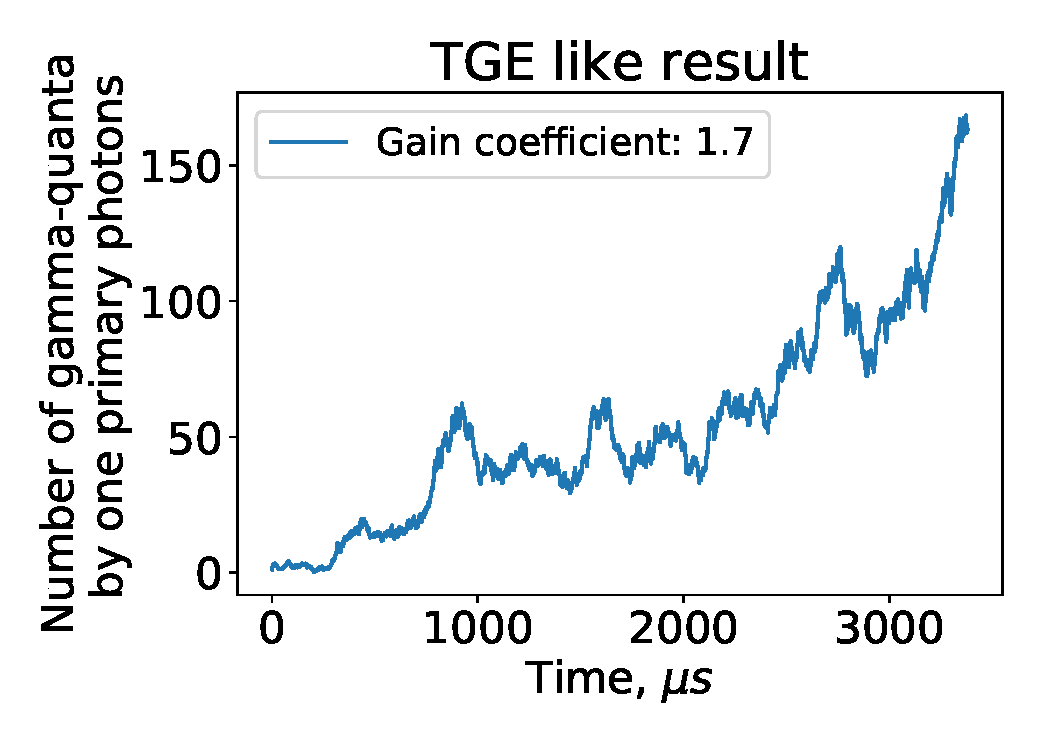
\includegraphics[width=0.95\linewidth]{figures/proofTGE.pdf}
		\caption{}
		\label{pic-tge-a}
	\end{subfigure}
	~
	\begin{subfigure}[b]{0.5\textwidth}
		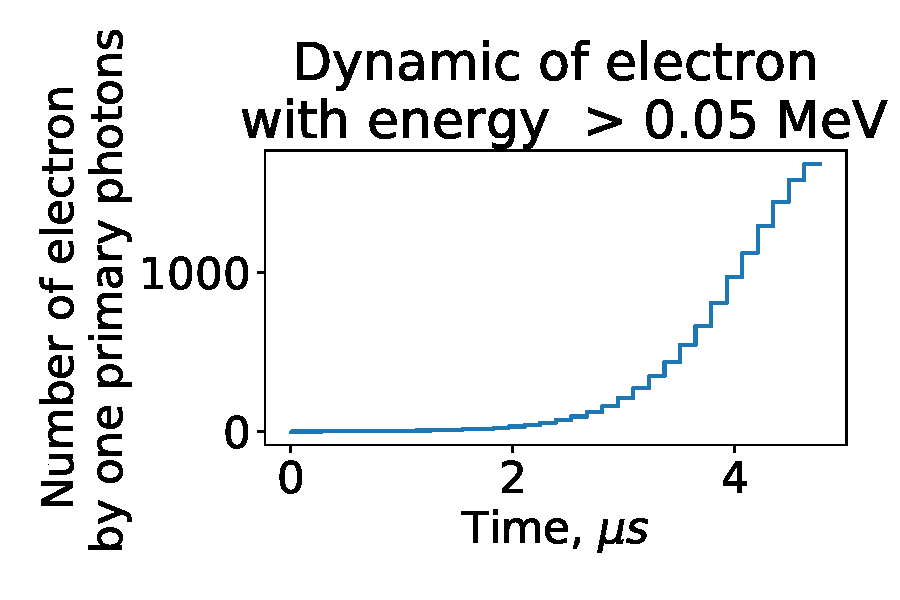
\includegraphics[width=0.95\textwidth]{figures/kotlinElectron.pdf}
		\caption{}
		\label{pic-electron-b}
	\end{subfigure}
	\caption{}
\end{figure}

\section{Perspectives}

\section{Conclusion}
\begin{itemize}
   	\item Reactor-like model is very good to describe TGF and other fast processes;
   	\item Slow processes like TGE could be described with additional assumptions about field dynamics;
   	\item The model could describe both TGE and TGF with the same mechanism depending on the state of the cloud.
\end{itemize}
Also reactor like model give next experimentally verifiable consequences:
\begin{itemize}
   	\item Contrary to Dweyer and unmodified Gurevitch models, reactor model predicts quasi-isotropic (according to field distribution) emittance of gamma-rays from a thundercloud.  	Measurement of the angular distribution of gamma-rays is required to prove or disprove the concept
   	
   	\item At first approximation, the energy spectrum of photons produced in RL model does not depend on radiation intensity (the spectrum depends on cell field and intensity on cell number).
\end{itemize}
Moreover reactor like TGE model can be used to investigate intercloud interaction.
\\
This work is supported by the Russian Science Foundation under grant No. 17-12-01439.
    
\bibliography{references}{}
\end{document}
